\chapter{Mobile Application Design}
\label{ch:mobile_app_design}

This chapter details the design of the mobile application developed for the Mountain Climber Health \& GPS Tracker system. Built using Flutter and Dart, the application provides climbers with real-time access to their health metrics, location data, and communication tools.

\section{Architecture}

The application follows a reactive architecture utilizing the standard Flutter widget tree paradigm combined with a robust state management solution.

\subsection{State Management}
The app employs the \textit{Provider} pattern for state management. This approach separates business logic from UI components, allowing different parts of the application to react to changes in BLE connection status, incoming sensor data, or new messages without requiring widespread widget rebuilds.

\section{BLE Scanning and Connection Flow}

The mobile application acts as a BLE Central device, scanning for and connecting to the Climber Main Device (acting as a BLE Peripheral).

\begin{figure}[H]
    \centering
    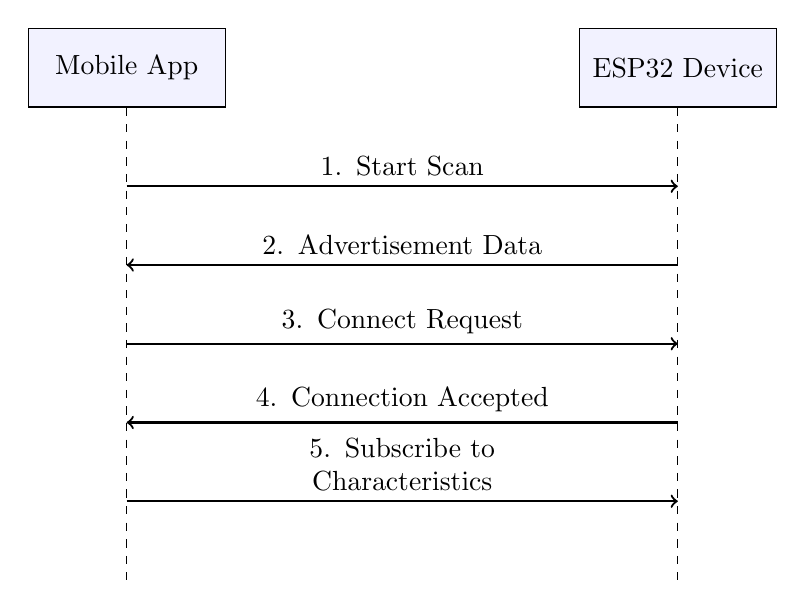
\begin{tikzpicture}[
        node distance=2cm,
        auto,
        box/.style={rectangle, draw, minimum width=2.5cm, minimum height=1cm, align=center, fill=blue!5},
        arrow/.style={->, thick}
    ]
    
    % Nodes
    \node[box] (app) {Mobile App};
    \node[box, right of=app, xshift=5cm] (device) {ESP32 Device};
    
    % Lifelines
    \draw[dashed] (app.south) -- +(0,-6cm);
    \draw[dashed] (device.south) -- +(0,-6cm);
    
    % Messages
    \draw[arrow] ([yshift=-1cm]app.south) -- node[above, text width=4cm, align=center] {1. Start Scan} ([yshift=-1cm]device.south);
    
    \draw[arrow] ([yshift=-2cm]device.south) -- node[above, text width=4cm, align=center] {2. Advertisement Data} ([yshift=-2cm]app.south);
    
    \draw[arrow] ([yshift=-3cm]app.south) -- node[above, text width=4cm, align=center] {3. Connect Request} ([yshift=-3cm]device.south);
    
    \draw[arrow] ([yshift=-4cm]device.south) -- node[above, text width=4cm, align=center] {4. Connection Accepted} ([yshift=-4cm]app.south);
    
    \draw[arrow] ([yshift=-5cm]app.south) -- node[above, text width=4cm, align=center] {5. Subscribe to Characteristics} ([yshift=-5cm]device.south);
    
    \end{tikzpicture}
    \caption{BLE Connection Sequence Diagram}
    \label{fig:ble_sequence}
\end{figure}

\subsection{Error Handling and Reconnection Strategy}
Mountainous environments are prone to interference that can drop BLE connections. The application implements an exponential backoff strategy for reconnection. If the connection drops, the app attempts to reconnect immediately. If that fails, it waits 2 seconds, then 4 seconds, up to a maximum interval, ensuring that battery life is not drained by continuous aggressive polling.

\section{Key Screens and UI Design Principles}

The UI is designed with high contrast and large touch targets, considering that climbers may be operating the app under harsh lighting conditions or while wearing gloves.

\subsection{Home Screen}
The Home screen serves as a dashboard summarizing the climber's status. It indicates the current BLE connection state and provides quick access to vital metrics and active alerts.

\begin{figure}[htbp]
    \centering
    
\includegraphics[width=0.8\textwidth]{app_home.png}
    \caption{Mobile App - Home Screen Interface}
    \label{fig:app_home}
\end{figure}

\subsection{Vitals Screen}
Displays real-time readings of Heart Rate, SpO2, and ambient temperature. Gauges and charts are used to show trends over time. Thresholds are color-coded (e.g., green for normal, red for critical).

\subsection{Map Screen}
Utilizes a custom painter in Flutter to render a specialized distance map. This map does not rely on internet map tiles (which are unavailable offline) but plots the relative positions of the user, the base camp, and other climbers based on received GPS coordinates and Haversine distance calculations.

\subsection{Messages Screen}
Provides a chat-like interface for two-way text messaging. Messages typed here are sent via BLE to the Climber Main Device, which relays them over the LoRa mesh network to the base camp or other climbers.

\section{Platform-Specific Configurations}

To utilize Bluetooth hardware, platform-specific permissions must be explicitly requested.

\subsection{Android Manifest}
The \texttt{AndroidManifest.xml} requires permissions for scanning, connecting, and accessing location (historically required for BLE scans on Android).
\begin{lstlisting}[language=XML, caption={Android BLE Permissions}, label={lst:android_permissions}]
<uses-permission android:name="android.permission.BLUETOOTH_SCAN" android:usesPermissionFlags="neverForLocation" />
<uses-permission android:name="android.permission.BLUETOOTH_CONNECT" />
<uses-permission android:name="android.permission.ACCESS_FINE_LOCATION" />
\end{lstlisting}

\subsection{iOS Info.plist}
The iOS \texttt{Info.plist} must include usage descriptions explaining to the user why Bluetooth is required.
\begin{lstlisting}[language=XML, caption={iOS Info.plist BLE Usage Description}, label={lst:ios_permissions}]
<key>NSBluetoothAlwaysUsageDescription</key>
<string>This app requires Bluetooth to connect to the climber health tracker.</string>
<key>NSBluetoothPeripheralUsageDescription</key>
<string>This app requires Bluetooth to communicate with the tracker.</string>
\end{lstlisting}
